\documentclass[a4paper,11pt,twoside,openany,fleqn]{memoir} % gebruik A4 papier, 11pt lettergrootte, en een apparte titelpagina. Een nieuw hoofdstuk begint op eender welke kant (links of rechts). Vergelijkingen komen op een kleine identatie van de linker kant, en de nummering staat rechts
% Template voor een LaTeX thesis op ESAT. 
% Auteur: Dirk Van Hertem: dirk.vanhertem@ieee.org
% Verander eraan wat je wil, en stuur opmerkingen door, dan houd ik de
% versie up to date
% lees README voor meer uitleg, of kijk naar http://homes.esat.kuleuven.be/~dvherten/esatthesis.html

%%%%%%%%%%%%%%%%%%%%%%%%%%%%%%%%%
% Maak de titelpagina
%%%%%%%%%%%%%%%%%%%%%%%%%%%%%%%%%

\newcommand{\NAAM}{Steven Janssens}
\newcommand{\NAAMb}{Vincent Renkens}% ook titelpagina.tex aanpassen als je dit invult (% teken weghalen)
\newcommand{\TITEL}{Taalverwerking door robots}
\newcommand{\SUBTITEL}{}
\newcommand{\PROMOTOR}{Prof.\,dr.\,Hugo Van Hamme}
%\newcommand{\PROMOTORb}{Prof.\,dr.\,Weet~Ook~Alles}% ook titelpagina.tex aanpassen (% teken weghalen)
\newcommand{\RICHTING}{Burgerlijk elektrotechnisch ingenieur (Ingebedde Systemen en Multimedia)}
\newcommand{\BEGELEIDER}{ir.\,Jort Florent Gemmeke}
\newcommand{\JAAR}{2013---2014}
\newcommand{\BEGELEIDERb}{ir.\,Bart Ons}% ook titelpagina.tex aanpassen (% teken weghalen)


%%%%%%%%%%%%%%%%%%%%%%%%%%%%%%%%%
% Header file
%%%%%%%%%%%%%%%%%%%%%%%%%%%%%%%%%
% filename: header_esat.tex
% auteur: Dirk Van Hertem (dirk.vanhertem@ieee.org)
% deze  file zorgt dat de juiste  opties gezet zijn. Een  aantal opties staan niet  default, maar ik
% raad je aan ze eens te bekijken, en indien gewenst te gebruiken.


\tightlists % weinig extra witruimte bij opsommingen (memoir optie)

\usepackage[english,dutch]{babel} % nederlandse tekstopmaak % english
                                % toegevoegd in versie 0.4

\usepackage{graphicx} % Gebruik figuren
\graphicspath{{figuren/}}
\usepackage{tabularx} % maak een tabel met een bepaalde breedte (gebruikt in symbolenlijst.tex)
\usepackage{microtype} % toegevoegd in versie 0.4
\usepackage{ifthen}% toegevoegd in versie 0.5
\usepackage{calc}% nieuw in 0.6b om te kunnen rekenen in deze header
% \newboolean{fourierfont} % nieuw in versie 0.6b, op aanraden van Benoit Willems, naar 2009 toe zou ik
%                          % fourier  standaard willen zetten, maar  voorlopig nog niet  om geen grote
%                          %   veranderingen   te   krijgen    vlak   voor   de   deadline.   Vervangt
% % \usepackage{fourier} in commentaar ==> werkt nog niet, voor de volgende keer...
% \setboolean{fourierfont}{true}

% %\ifthenelse{\boolean{fourierfont}}{%

%%%%%%%%%%%%%%%%%%%%%
%%% Als je fourier wilt, uncomment de volgende regio:
%%%%%%%%%%%%%%%%%%%%%
%\makeatletter
%\let\my@@font@warning\@font@warning
%\let\@font@warning\@font@info
%\makeatother%
%\usepackage{fourier}%
%\makeatletter
%\let\@font@warning\my@@font@warning
%\makeatother

%%%%%%%%%%%%%%%%%%%%%
% inputenc
%%%%%%%%%%%%%%%%%%%%
% inputenc is afhankelijk van uw systeem (en os). Waarschijnlijk maakt
% een van de volgende \usepackage[]{inputenc} dat alles goed
% opgeslagen kan worden. Waarschijnlijk heb je latin1 nodig. \'e werkt altijd...

%\usepackage[latin1]{inputenc} % zorgt dat je ook � � en dergelijke kan ingeven
%\usepackage[utf8]{inputenc} % zorgt dat je ook � � en dergelijke kan ingeven

%%%%%%%%%%%%%%%%%%%%
% andere mogelijk nuttige pakketten
%%%%%%%%%%%%%%%%%%%%

% \usepackage{subfig}   % Gebruik subfiguren
% \usepackage{color}    % Gebruik kleuren
% \usepackage{icomma}   % zet de spati�ring goed bij kommagetallen (Europeese notatie)
% \usepackage{amssymb,amsmath,amsfonts} % extra wiskundige symbolen en
% constructies
% \usepackage{eurosym}  % \euro geeft het euroteken
% \usepackage{cite}     % verbetert de weergave van citaties 
% \usepackage{listings} % om code toe te voegen in uw document
% \usepackage{booktabs} % toegevoegd in version 0.4


% De volgende opties bepalen hoe figuren op een blad geplaatst moeten worden. Lees het volgende document voor meer informatie: http://www.ctan.org/tex-archive/info/epslatex.pdf

\setcounter{topnumber}{4}
\setcounter{bottomnumber}{4}
\setcounter{totalnumber}{10}
\renewcommand{\textfraction}{0.15}
\renewcommand{\topfraction}{0.85}
\renewcommand{\bottomfraction}{0.70}
\renewcommand{\floatpagefraction}{0.66}

% Opmerking: het volgende  stuk definieert de pagina opmaak. Indien de  keuze energie genomen wordt,
% dan wordt een opmaak met anderhalve regelafstand  genomen. Ofdat dit zinvol is, dat laat ik in het
% midden, de mensen die twijfelen lezen best de volgende url:
% http://www.tex.ac.uk/cgi-bin/texfaq2html?label=linespace. 
% De opmaak van energie heeft ook iets minder witruimte aan de randen. 
% Veranderen van opmaak kan simpelweg door de  waarde van \energie (zie regel na deze commentaar) de
% waarde "true" of "false" te geven.
\newboolean{energie}
\setboolean{energie}{false}

\ifthenelse{\boolean{energie}}% versie 0.6
{% deze optie is ook versie 0.6
% zet de pagina op (zie memman.pdf p 66)
\settrimmedsize{297mm}{210mm}{*}%
\setlength{\trimtop}{0pt}%
\setlength{\trimedge}{\stockwidth}%
\addtolength{\trimedge}{-\paperwidth}%
\settypeblocksize{654pt}{455pt}{*}% Van 634 naar 694 pt in versie 0.7
\setulmarginsandblock{2cm+\onelineskip+1.5\onelineskip}{2.65cm}{*}% Aanpassing 0.7
\setlrmargins{*}{*}{0.9}% verhouding buitenkantmarge/rugmarge. Verzet
% van 1.5 naar 0.9 vanaf versie 0.4
\setmarginnotes{17pt}{51pt}{\onelineskip}%
\setheadfoot{\onelineskip}{2\onelineskip}%
\setheaderspaces{*}{1.5\onelineskip}{*}% Aangepast versie 0.7
%
%zorg ervoor dat TOC niet te breed wordt:
%\setpnumwidth{2.5em}
%\setrmarg{3em} 
%
\checkandfixthelayout%
\OnehalfSpacing%
}%
{%
% zet de pagina op (zie memman.pdf p 66)
\settrimmedsize{297mm}{210mm}{*}%
\setlength{\trimtop}{0pt}%
\setlength{\trimedge}{\stockwidth}%
\addtolength{\trimedge}{-\paperwidth}%
\settypeblocksize{634pt}{448.13pt}{*}%
\setulmargins{4cm}{*}{*}%
\setlrmargins{*}{*}{0.9}% verhouding buitenkantmarge/rugmarge. Verzet
% van 1.5 naar 0.9 vanaf versie 0.4
\setmarginnotes{17pt}{51pt}{\onelineskip}%
\setheadfoot{\onelineskip}{2\onelineskip}%
\setheaderspaces{*}{2\onelineskip}{*}%
%
%zorg ervoor dat TOC niet te breed wordt:
%\setpnumwidth{2.5em}
%\setrmarg{3em} 
%
\checkandfixthelayout%
}
\setlength{\parindent}{0pt}
\setlength{\parskip}{0.5\baselineskip}
\setlength{\cftbeforechapterskip}{0pt}

% Voor de nummeringsdiepte te veranderen: met level 4 nummer je ook subsecties
\setcounter{secnumdepth}{4} % default gemaakt in versie 0.4
%\setcounter{tocdepth}{4}
\usepackage[hypertexnames=false]{hyperref} % geeft links zodat je een
                                % interactief document krijgt (zeer
                                % interessant als je het ooit online
                                % zet) 

% % caption maar 0.8  \textwidth breed maken, en normaal lettertype (dit was reeds  zo, maar nu kun je
% % zien wat je kan veranderen indien nodig) (versie 0.7)
% \changecaptionwidth
% \captionwidth{0.8\textwidth}
% %\normalcaptionwidth
% \captiontitlefont{\normalsize} ==> werkt nog niet, later nog eens zien

\usepackage{memhfixc}  % anders krijg je een error (memoir samen met hyperref...)

%%% Local Variables: 
%%% mode: latex
%%% TeX-master: "eindwerk_template"
%%% End: 


\begin{document}
%\selectlanguage{english}%indien de thesis in het engels wordt gemaakt
\selectlanguage{dutch}% voor normale thesissen

\vspace*{-1cm}\hspace*{-1cm}
\begin{minipage}{0.5\textwidth}
\textsc{Faculteit}\\ \textsc{Ingenieurswetenschappen}\\
\\
\textsc{Departement}\\
\textsc{Elektrotechniek -- ESAT}
\end{minipage}\hfill%
\ifthenelse{\boolean{energie}}{%extra  stuk  uit  versie  0.5a,  om te  compenseren  voor  de  gekke
                               %plaatsing van de sedes (met dank aan Joost Busschaert). Tijdelijke fix
\begin{minipage}{0.2\textwidth}
 \begin{flushright}
 
\includegraphics[width=2cm]{sedes}
 \setlength{\unitlength}{1mm}
 \begin{picture}(28.5,2)
  \put(0,0){\line(1,0){28.5}}
 \end{picture}
 KATHOLIEKE\\UNIVERSITEIT\\LEUVEN
 \end{flushright}
 \end{minipage}
}{\begin{minipage}{0.3\textwidth}
 \begin{flushright}
 
\includegraphics[width=2cm]{sedes}
 \setlength{\unitlength}{1mm}
 \begin{picture}(28.5,2)
  \put(0,0){\line(1,0){28.5}}
 \end{picture}
 KATHOLIEKE\\UNIVERSITEIT\\LEUVEN
 \end{flushright}
 \end{minipage}
}

\vfill
\pagestyle{empty}

\begin{center}
\begin{Huge}
\textsf{\TITEL}\\[4mm]
\end{Huge}
\begin{LARGE}
  \textsf{\SUBTITEL}
\end{LARGE}
\end{center}
\vfill
\begin{tabular}{p{0.49\textwidth}p{0.5\textwidth}}
   & Eindwerk voorgedragen tot het behalen van het diploma van
   \RICHTING\\
   & \\
   & \begin{Large}\textbf{\NAAM}\end{Large}\\
   & \begin{Large}\textbf{\NAAMb}\end{Large}\\
   & \\
   & Promotor:\\
   & \hspace{4mm}\begin{large}\PROMOTOR\end{large}\\
%  & \hspace{4mm}\begin{large}\PROMOTORb\end{large}\\
   & Dagelijkse begeleiding:\\
   & \hspace{4mm}\begin{large}\BEGELEIDER\end{large}\\
   & \hspace{4mm}\begin{large}\BEGELEIDERb\end{large}\\
\end{tabular}
\\
\\
\\
\begin{center}
\JAAR
\end{center}

\cleardoublepage

%%% Local Variables: 
%%% mode: latex
%%% TeX-master: "eindwerk_template"
%%% End: 


\pagenumbering{roman}
\pagestyle{plain} %%%% hier toevoegen 
\begin{otherlanguage}{dutch}
\begin{small}\vspace*{\fill} \copyright\ Copyright K.U.Leuven\\
\\
Zonder voorafgaande schriftelijke toestemming van zowel de
promotor(en) als de auteur(s) is overnemen, kopi\"eren, gebruiken of
realiseren van deze uitgave of gedeelten ervan verboden. Voor
aanvragen tot of informatie i.v.m. het overnemen en/of gebruik
en/of realisatie van gedeelten uit deze publicatie, wend U tot de
K.U.Leuven, Departement Elektrotechniek -- ESAT, Kasteelpark
Arenberg 10, B-3001 Heverlee (Belgi\"e). Telefoon~\mbox{+32-16-32 11
30} \& Fax.~\mbox{+32-16-32 19 86} of via email: \url{info@esat.kuleuven.be}.

Voorafgaande schriftelijke toestemming van de promotor(en) is
eveneens vereist voor het aanwenden van de in dit afstudeerwerk
beschreven (originele) methoden, producten, schakelingen en
programma's voor industrieel of commercieel nut en voor de
inzending van deze publicatie ter deelname aan wetenschappelijke
prijzen of wedstrijden.
\end{small}
\end{otherlanguage}
\vspace*{3cm}

\begin{otherlanguage}{english}
\begin{small}
\copyright\ Copyright by K.U.Leuven\\
\\
Without written permission of the promotors and the authors it is
forbidden to reproduce or adapt in any form or by any means any
part of this publication. Requests for obtaining the right to
reproduce or utilize parts of this publication should be addressed
to K.U.Leuven, Departement Elektrotechniek -- ESAT, Kasteelpark
Arenberg 10,  B-3001 Heverlee  (Belgium). Tel.~\mbox{+32-16-32 11
30}   \& Fax.~\mbox{+32-16-32 19 86} or by email: \url{info@esat.kuleuven.be}.

A written permission of the promotor is also required to use the
methods, products, schematics and programs described in this work
for industrial or commercial use, and for submitting this
publication in scientific contests.
\end{small}
\end{otherlanguage}

% \selectlanguage{dutch}

%%% Local Variables: 
%%% mode: latex
%%% TeX-master: "eindwerk_template"
%%% End: 
 % deze file zit al in de zip-file zitten

% include de volgende gedeelten per hoofdstuk. Werk best niet vanuit 1 file


\chapter*{Voorwoord}
\addcontentsline{toc}{chapter}{Voorwoord}
\label{cha:voorwoord}

%%% Local Variables: 
%%% mode: latex
%%% TeX-master: "eindwerk_template"
%%% End: 

\chapter*{Abstract}
\addcontentsline{toc}{chapter}{Abstract}

%%% Local Variables: 
%%% mode: latex
%%% TeX-master: "eindwerk_template"
%%% End: 

\tableofcontents\clearpage

\chapter*{Lijst van symbolen}
\addcontentsline{toc}{chapter}{Lijst van symbolen}

\begin{center}
  \begin{tabularx}{0.8\textwidth}{p{1.5cm}X}
    $\pi$ & het getal pi\\
    $42$  & The Answer to the Ultimate Question of Life, the Universe, and Everything\cite{h2g2}
  \end{tabularx}
\end{center}
%%% Local Variables: 
%%% mode: latex
%%% TeX-master: "eindwerk_template"
%%% End: 
\clearpage
\def\listfigurename{Lijst van figuren}
\listoffigures\clearpage
\def\listtablename{Lijst van tabellen}
\listoftables
%\def\lstlistlistingname{Lijst van codeblokken}

\cleardoublepage
\pagenumbering{arabic}
\pagestyle{ruled}


\chapter{Inleiding}
\label{cha:inleiding}


\chapter{Masterframe}
\label{cha:masterframe}

In dit hoofdstuk zal er een masterframe opgebouwd worden zoals beschreven in \cite{Tessema}. Vooraf moet er nagedacht worden over wat de robot allemaal kan en hoe die dan zou aangestuurd kunnen worden door een gebruiker. Uit deze lijst van mogelijke spraakcommando's (komende uit de natuurlijke taal) zal dan een masterframe opgesteld worden zodat de commando's hierarchisch gestructureerd worden. De robot is te zien in Figuur ~\ref{fig:robot}. Deze kan vooruit en achteruit rijden, draaien en met de grijper vooraan kan hij objecten oppakken. Bovendien heeft de robot een aantal sensoren om objecten te detecteren en om aan tracking te doen. \\

\begin{figure}[h]
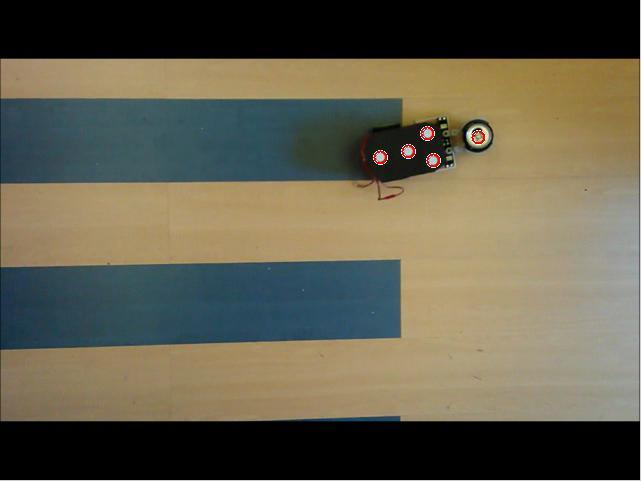
\includegraphics[width=0.5\textwidth]{robot.jpg}
\label{fig:robot}
\centering
\caption{Foto van de gebruikte robot}
\end{figure}

\section{Frames}
\label{sec:frames}

De eenvoudigste opdrachten die een gebruiker de robot zou kunnen geven is om te bewegen. Enkele voorbeelden hiervan zijn '\textit{ga naar daar}' of '\textit{rij 5cm vooruit}'. Er wordt hier onderscheid gemaakt tussen drie soorten bewegingen:

\begin{itemize}
\item een absolute beweging: dit is een beweging naar een vast punt in het frame zoals bv. de hoek of het midden. Dit zou ook een object kunnen zijn.
\item een relatieve beweging: dit is een beweging relatief ten opzichte van zijn huidige positie zoals een bepaalde afstand voorruit of naar links rijden. 
\item bewegen voor een bepaalde tijd: dit kan zijn tot de gebruiker stop zegt of voor een bepaalde tijdsduur.
\end{itemize}

Elke soort van de opgesomde bewegingen kan een rotatie en/of een translatie bevatten.  \\
\\
Andere commando's zijn commando's waarvoor de robot zijn grijper nodig heeft. Dit zouden eenvoudige dingen kunnen zijn zoals '\textit{grijp}' of '\textit{laat los}'. Voor deze commando's moet de robot maar \'e\'en actie uitvoeren, namelijk zijn grijper sluiten of openen. Er zijn echter ook complexere commando's zoals '\textit{breng het blikje naar de bal}'. Hiervoor moet de robot verschillende dingen doen; hij moet het blikje vinden, naar het blikje rijden, het blikje pakken, de bal vinden, naar de bal rijden en zijn grijpers openen om het blikje los te laten.\\
\\
Uit de bovenstaande beschrijving wordt er een mogelijke lijst van commando's gehaald. Dit zijn de frames in onze masterframe. Deze zijn te zien in tabel \ref{tab:commands}.

\begin{table}[h]
\centering
\begin{tabular}{| l | l |}
\hline
\textbf{move\_rel} &  bewegen relatief ten opzichte van de huidige positie\\
\textbf{move\_abs} & bewegen naar een vast punt in het frame\\
\textbf{move\_to\_obj} & bewegen naar een object\\
\textbf{move\_time} & bewegen voor een bepaalde tijd\\
\textbf{turn\_abs} & zich richten naar een bepaalde richting\\
\textbf{turn\_rel} & een bepaalde hoek draaien relatief ten opzichte van de huidige ori"entatie\\
\textbf{turn\_time} & draaien voor een bepaalde tijd\\
\textbf{grab} & grijpen met de grijpers\\
\textbf{release} & de grijpers openen\\
\textbf{grab\_obj} & een bepaald object pakken\\
\textbf{move\_obj} & een object verplaatsen naar een andere locatie\\
\textbf{stop} & stop de huidige actie\\
\hline
\end{tabular}
\caption{Lijst van commando's}
\label{tab:commands}
\end{table}

\section{Slots en slotvalues}
\label{sec:slots_slotvalues}

Voor alle commando's die opgesomd zijn in tabel \ref{tab:commands} moet er beslist worden welke parameters er moeten worden meegegeven met de commando's en welke waardes deze kunnen aannemen. De parameters worden de slots genoemd en de bijhorende waarden de slotvalues. Bij de keuze van deze parameters (en bijhorende waarden) is er rekening gehouden met de verwachte input. De commando's zouden immers op een zo natuurlijk mogelijke manier moeten kunnen gegeven worden. Een normale gebruiker zal bijvoorbeeld zelden zeggen: '\textit{rij naar positie met x-co"ordinaat 3 en y-co"ordinaat 5}' maar zal eerder iets zeggen als '\textit{rij naar het midden}'. Achteraf zal dit midden in het verdere programma wel co"ordinaten krijgen, maar dit heeft geen invloed voor de gebruiker.\\
\\
Voor de afstanden die de robot relatief ten opzichte van zijn huidige positie kan afleggen wordt er gekozen voor een exponentieel (of hi"erarchisch) verloop omdat voor kleine bewegingen van de robot een hogere precisie nodig is dan voor grotere bewegingen.\\
De robot kan ook bewegen naar vaste punten. Zoals al vermeld moeten deze punten benoembaar zijn in de natuurlijke taal e.g. 'het midden'. Daarom wordt voor de vaste posities gekozen voor het midden, de hoeken en het midden van de wanden. Deze plaatsen zullen benoemd worden zoals de windrichtingen zoals in Figuur ~\ref{fig:masterframe}.\\
Voor de acties waarbij de robot moet bewegen voor een bepaalde tijd moeten er verschillende duraties zijn, maar het moet ook mogelijk zijn om de robot te laten bewegen tot de gebruiker stop zegt (de rotatie kan zo bv gebruikt worden om de robot te richten). In dit laatste geval is het echter wel prefereerbaar om te robot traag te laten bewegen zodat deze niet te lang blijft door roteren door de inherente vertraging van de spraaksoftware. De tijden worden net zoals de afstanden exponentieel gekozen.\\
De hoeken die de robot moet kunnen draaien, moeten alsook in de natuurlijke taal benoemd kunnen worden. Logische keuze's zijn alvast $90^\circ$ en $180^\circ$ voor bv. 'draai naar links' of 'draai om'. $45^\circ$ is ook nog gekozen voor bv 'draai schuin naar rechts'.\\
Het absoluut richten van de robot moet mogelijk zijn naar alle 'windrichtingen'. De hoeken zijn dus gekozen van $0^\circ$ tot en met $315^\circ$ in stappen van $45^\circ$. Deze absolute hoeken worden gemeten ten opzichte van bv. de onderste plank van het frame waarin de robot beweegt.\\
\\
Met al deze gemaakte beslissingen kan nu het masterframe opgesteld worden. Deze is te zien in Figuur \ref{fig:masterframe}. De tijden worden hierin weergegeven in seconden en de afstanden in centimeter omdat met de huidige opstelling dit de meest waarschijnlijke dimensies zijn die uitgesproken zullen worden.

\begin{figure}[h]
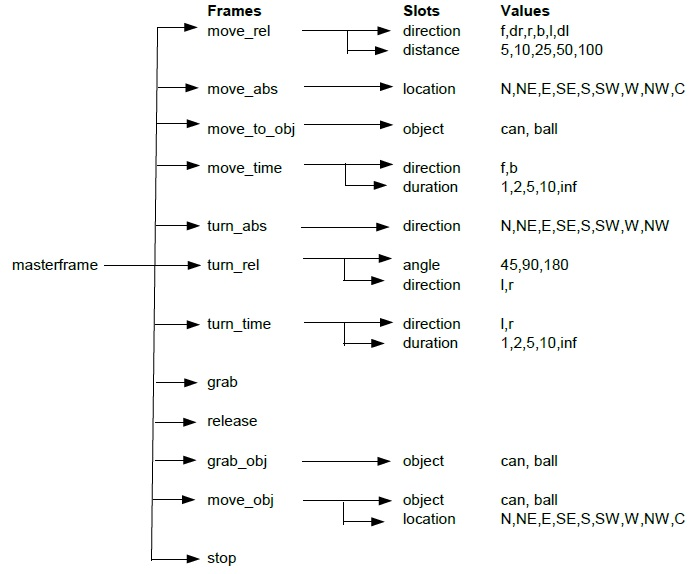
\includegraphics[width=\textwidth]{masterframe.jpg}
\label{fig:masterframe}
\centering
\caption{Het gekozen masterframe}
\end{figure}

%\include{besluit}


% \nocite{eenboek} % refereert naar eenboek, zonder dat er in de tekst naar verwezen wordt
% \nocite{*} % verwijst naar alles in uw bibfile zonder dat er naar verwezen moet worden in de tekst

\bibliographystyle{IEEEtran_nl}   %    citeren   zoals    door   ieee   aangeraden    wordt.   Leest
                                % IEEEtran_bst_HOWTO.pdf voor  meer inlichtingen. IEEEtran_nl is een
                                % aangepaste versie van IEEEtran, waarbij de bindwoorden, maanden en
                                % dergelijke in het nederlands gezet zijn.
%\bibliographystyle{IEEEtran} % originele versie, te gebruiken als je uw tekst in het engels doet 
\bibliography{referenties} %  maak een eindwerk.bib bestand aan met uw referenties (dit is iets waar je best direct mee begint en niet op het einde doet)


%\appendix % indien gewenst
%\include{appendix1}

\end{document}

%%% Local Variables: 
%%% mode: latex
%%% TeX-master: t
%%% End: 
